\documentclass[../Master.tex]{subfiles}
\begin{document}
\chapter{Result and discussion}

\section{Pyrazole Ligand Development}\label{sec:pyr-dev}

\subsection{Starting Materials}\label{sec:starting-materials}

While several ligands were synthesized and utilized within the research group led by Professor L. Carlucci, my specific contribution focused exclusively on one of these ligands, that is based upon an already studied one. The structure of the starting material, 4,4’-malonyldibenzoic, and the retrosynthetic approch to it is reported.

\begin{figure}[h]
	\centering
	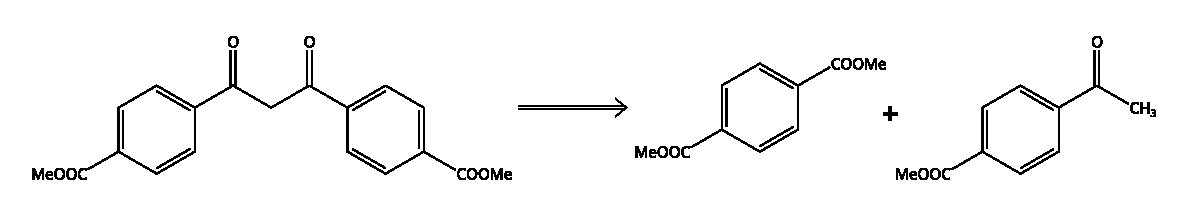
\includegraphics[width=16cm,height=8cm,keepaspectratio]{Structures/dikest2-retro.eps}
	\caption{4,4’-malonyldibenzoic acid Retrosynthesis Approach}\label{fig:dikest2-retro}
\end{figure}

The synthesis of the ligand is based on the cross-Claisen condensation, and the reaction was conducted with excellent yields and purity, resulting in the production of tens of grams of the compound. The reagents required for the synthesis are readily available commercially, facilitating the accessibility and reproducibility of the process. \\
The same synthetic approach has been carried out over a wide range of analogue compound, resulting tipically in high yield scalable reaction, as for example the ligand that will be analyzed in the section\ \ref{sec:electrochemistry} has been approached with the same strategies.
\newpage
\subsection{Pyrazole Formation}\label{sec:pyrazole-reaction}
Starting from the 1,3-diketone diester intermediate the apparently easier way to procede with the pyrazole formation is using hydrazine, of which a brief reaction mechanism is reported.

\begin{figure}[h!]
	\centering
	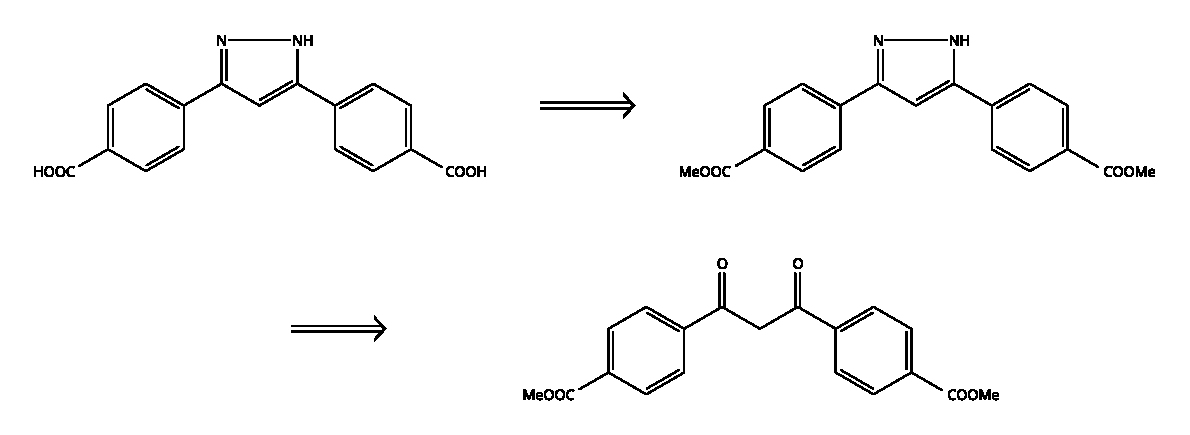
\includegraphics[width=16cm,height=8cm,keepaspectratio]{Structures/pyrazole-retro.eps}
	\caption{Pyrazole Ligand Retrosynthesis}\label{fig:pyrazole-retro}
\end{figure}
Typically the reaction reaches completion in ethanol under reflux conditions with an excess of hydrazine within a few hours withouth any catalyzer: in this specific case several problems has been encountered and analyzed.

\begin{figure}[h!]
	\centering
	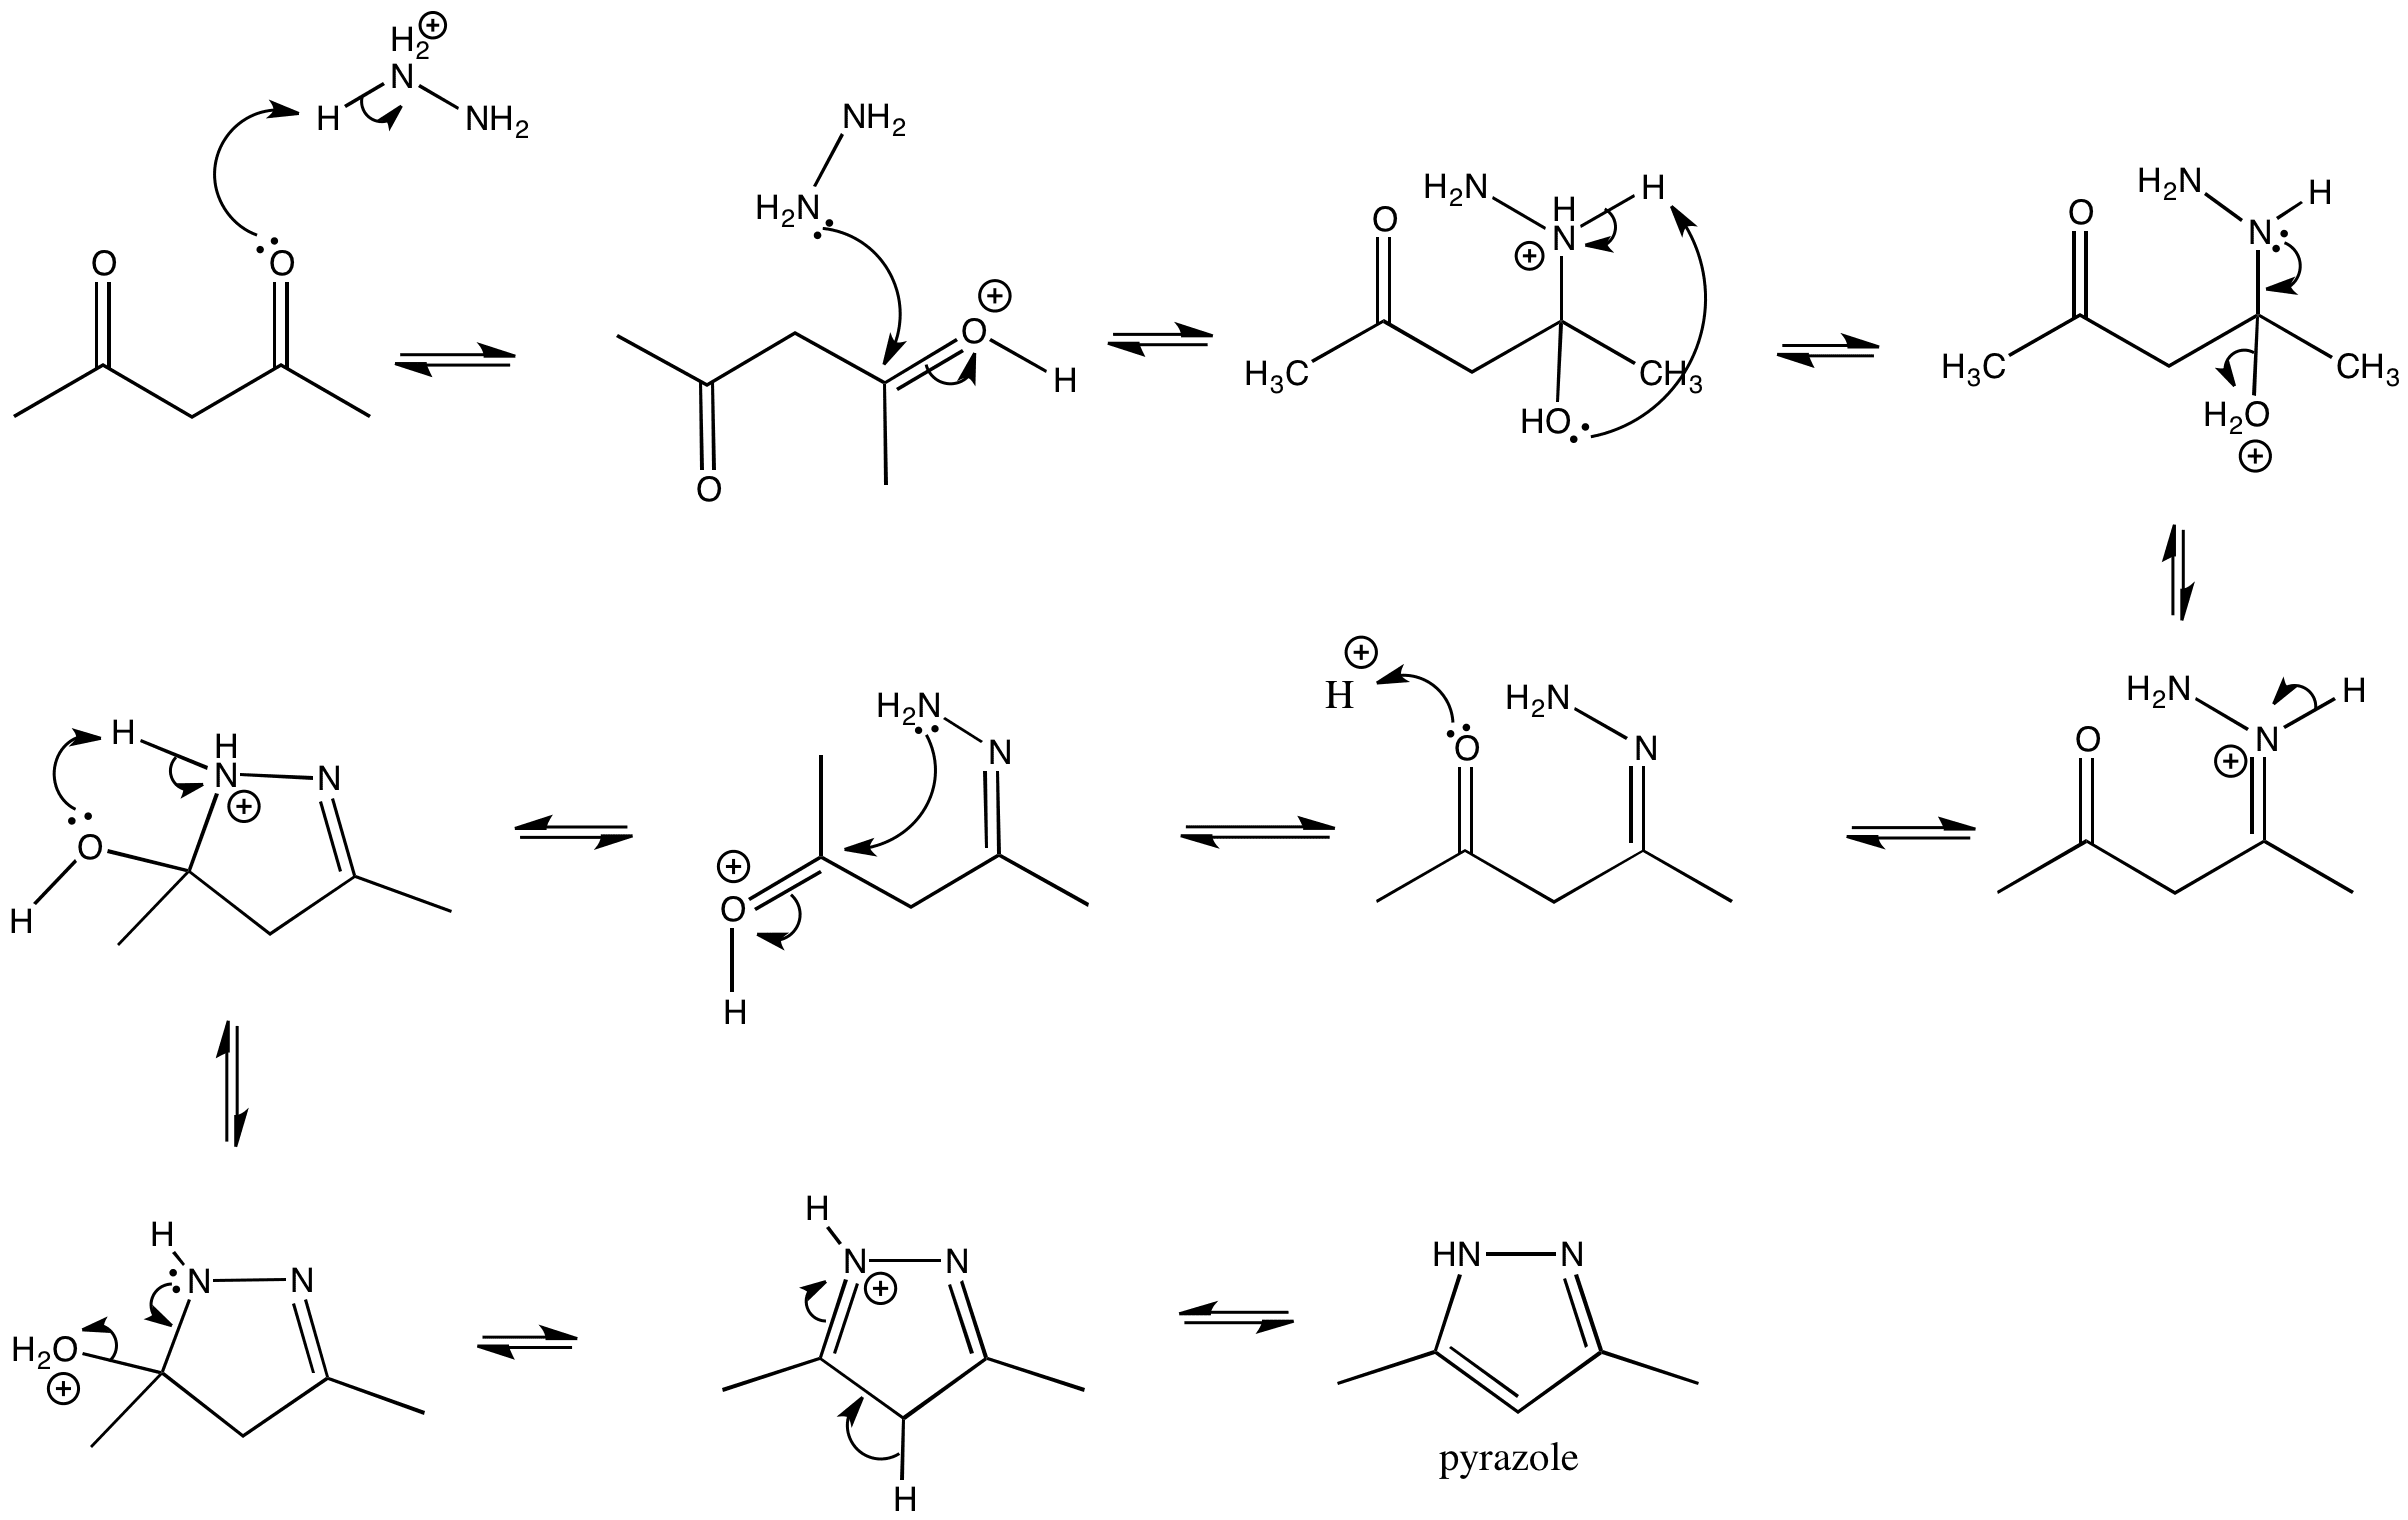
\includegraphics[width=16cm,height=8cm,keepaspectratio]{Images/pyrazole-mechanism.png}
	\caption{Pyrazole Formation Mechanism}
\end{figure}

\subsubsection{Solvent Choice and Reagent Solubility}\label{sec:solvent}

Dimethyl 4,4’-malonyldibenzoate is poorly soluble in most organic solvents, even after careful grinding and sonication. Different alternatives has been evaluated, noting that the solvent choice was highly restricted from the fact that 65\% hydrazine in water has been initially used. \\
Given the relatively low polarity of the ester functionalities, it would be beneficial to use a less polar solvent that still allows for the formation of a single phase with hydrazine water solution, while avoiding reactions with it.\\
The so low solubility can be attributed to several characteristic of the compound that is an highly simmetric diester. The correlation between solubility and symmetry of a molecule can vary depending on various factors, including the specific nature of the molecule and the solvent in which it is dissolved. While symmetry can influence certain aspects of a molecule's behavior, such as its physical properties, there is no general rule or direct correlation between solubility and symmetry. For example, symmetric molecules may have a more compact shape, which could reduce the surface area available for interaction with the solvent molecules. This can potentially lead to lower solubility if the solvent relies on surface interactions for dissolution. On the other hand, highly symmetrical molecules may have fewer polar or charged groups, which can reduce their ability to form favorable interactions with polar solvents. Other factors, such as temperature, pressure, and the presence of specific functional groups, can also significantly impact solubility. Experimental data and detailed analysis of the specific compound of interest are often required to accurately determine its solubility characteristics.\\
For these reasons the use of different solvent has been investigated, involving different approch for product recovery subsequently to solvent properties. \\
Reaction conducted in EtOH gives below 30\% yield and overnight reaction time is needed to observe appreciable product formation. Nevertheless the solvent was easily removable by evaporation and the product can be easily purified afterward.\\
The use of THF as solvent gives no noticeable advantages in solubility or product recovery, providing lower yield than former conditions.\\
DMSO on the other hand provided higher yield of approximately 50\%, at the cost of highly time expensive and difficult recovering, as the product itself it highly soluble in the solvent. High diluition in water of the reaction mixture was carried out, followed by several centrifugation phases. This process was considered not reproducible and difficult to carry out especially on higher scale reaction. The valuable aspect of DMSO use are high reactant solubility and the possibility to achieve higher reaction temperature.\\
Trying to avoid extreme water diluition and centrifugation as recovery option DMF was tested as solvent, noting the fact that DMF can be evaporated. The solubility of the reactant is not as great as in DMSO but better than EtOH or THF and higher temperature is possible too. Despite the promising outlook the result are not as expected and the observed yield is not higher than 30\%.\\
In light on the obtained information, it is worth to make a few assessments and adjustments.

\subsubsection{Purification Methodes}\label{sec:pyr-purification}

The ideal purification method should be selective, efficient, scalable with minor side effects. Keeping in mind this preamble some alternative regarding the purification step has benn evaluated.

\begin{enumerate}
	\item  Gravity Chromatographic Column, Hex:AcOEt 75:25

	      Through this process small quantities high purity product has been obtained. The operations itself is not time efficient and takes up large amount of solvent, leaving behind a considerable quantity of product of interest.\\
	      Backing up this consideration, several examples of chromatographic column purification of similar pyrazole compounds are reported in the literature, but none of them use considerable amount of products.
	\item Recrystallization from EtOH

	      Taking special care to hot filter on Teflon filter any residual unreacted reagents reactants and conducting controlled cooling, a product of good purity is obtained in a reasonable time and using a minimum amount of solvent. \\
	      Recrystallization from EtOH results frequently in the literature (https://doi.org/10.1515/HC.2004.10.2-3.249) as a purification method for pyrazole compounds.
	\item Soxhlet with EtOH

	      The technique appears to be of good efficiency in terms of purity but the amount of solvent and time required are excessive. The long time in contact with EtOH partially causes the dissolution of some of the impurities. It might be appropriate on large amounts of product where
	      crystallization becomes less efficient.
\end{enumerate}
\subsection{Pyrazole Ester Hydrolisis}\label{sec:pyrazole-hydro}

The removal of methyl esters is a standard practice in organic chemistry, and no specific issues were encountered during this step of the synthesis: two sythetic pathway as been analyzed.\\
Removal using LiOH in THF:H$_2$O 1:1 has been initially utilized, but the yield from different reaction was not highly reproducible, maybe for the precence of different impurity deriving from different pyrazole synthesis method.\\
Instead, removal with NaOH in MeOH:H$_{2}$O 1:1 gives better results, with higher yield.

\subsection{Alternative Pyrzole Synthesis}\label{sec:alt-pyrazole-synthe}

Considering the problem encountered in exploring the synthesis of this ligand, another synthetic route could be followed, using a croton condensation and then a conjugate addition to the newly formed alpha beta unsaturated compound.

\begin{figure}[h!]
	\centering
	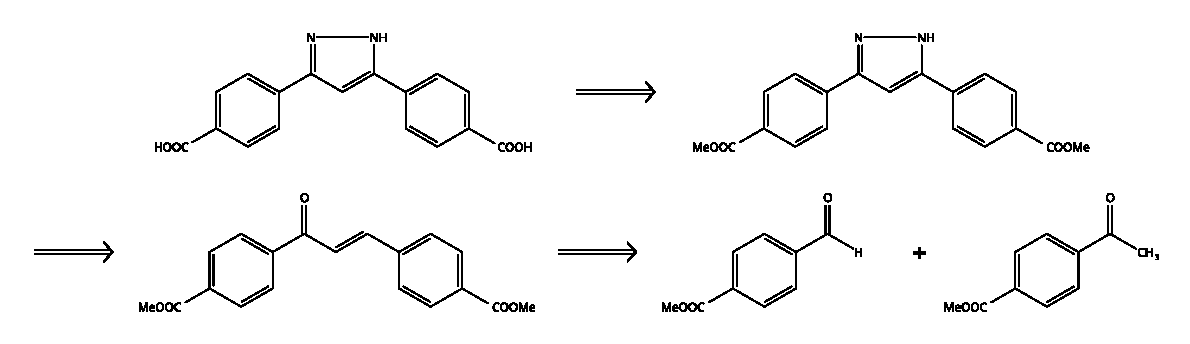
\includegraphics[width=16cm,height=8cm,keepaspectratio]{Structures/pyrazole-retro-alt.eps}
	\caption{Pyrazole Ligand Alternative Retrosynthesis}\label{fig:pyrazole-retro-alt}
\end{figure}

\section{Electrochemistry}\label{sec:electrochemistry}

\subsection{Why electrochemistry on these molecules?}\label{sec:elect-intro}

Cyclic voltammetry (CV) is a technique used in the analysis of organic and inorganic compounds\ \cite{elgrishi_practical_2018}. It provides information about reduction and oxidation processes of molecular species, the stability, the conversion and storage of energy and several other interesting properties. CV is also invaluable to study electron transfer-initiated chemical reactions, which includes catalysis. CV can be used to estimate the electron affinity and ionization energy of test compounds in a much cheaper and faster way compared to other high vacuum methods. It is important in electrochemistry because it allows to study the electron transfer processes that are at the center of the reactivity of inorganic complexes.
The aforementioned parameters correlate with the energy levels of highest occupied molecular orbital (HOMO) and lowest unoccupied molecular orbital (LUMO).

When cyclic voltammetry (CV) is combined with or ultraviolet-visible and near-infrared (UV-Vis-NIR) spectroscopies, it provides useful information such as electron affinity, ionization potential, band-gap energies, the type of charge carriers, and degradation information\ \cite{pluczyk_using_2018}. Analizing the CV experiment data is possible to determine the band-gap value that can be later evaluted against the one obtained from the spectroscopic UV data.

\end{document}

%%% Local Variables:
%%% mode: latex
%%% TeX-master: "../Master"
%%% End:

